\documentclass{sigchi}

% Remove or comment out these two lines for final version
\toappear{
Permission to make digital or hard copies of all or part of this work for personal or classroom use is granted without fee provided that copies are not made or distributed for profit or commercial advantage and that copies bear this notice and the full citation on the first page. To copy otherwise, or republish, to post on servers or to redistribute to lists, requires prior specific permission and/or a fee.

Gamification’13, October 2 – 4, 2013, Stratford, ON, Canada.

Copyright 2013 ACM 978-1-XXXX-XXXX-X/XX/XX...\$10.00.
}

\pagenumbering{arabic}% Arabic page numbers for submission. 

% Use \toappear{...} to override the default ACM copyright statement (e.g. for preprints).

% Load basic packages
\usepackage{balance}  % to better equalize the last page
\usepackage{graphicx} % for EPS, load graphicx instead
\usepackage{times}    % comment if you want LaTeX's default font
\usepackage{url}      % llt: nicely formatted URLs

\usepackage{subfigure}
\graphicspath{{figures/}}

% llt: Define a global style for URLs, rather that the default one
\makeatletter
\def\url@leostyle{%
  \@ifundefined{selectfont}{\def\UrlFont{\sf}}{\def\UrlFont{\small\bf\ttfamily}}}
\makeatother
\urlstyle{leo}

% To make various LaTeX processors do the right thing with page size.
\def\pprw{8.5in}
\def\pprh{11in}
\special{papersize=\pprw,\pprh}
\setlength{\paperwidth}{\pprw}
\setlength{\paperheight}{\pprh}
\setlength{\pdfpagewidth}{\pprw}
\setlength{\pdfpageheight}{\pprh}

%% Puts space after macros, unless followed by punctuation
\usepackage{xspace}

%%% Personal macros
%% Tired of typing CO2 so many times, requires xspace package
\newcommand{\COtwo}{CO\ensuremath{_2}\xspace}
%% Hawai`i with okina
\newcommand{\Hawaii}{Hawai`i\xspace}
%% Hawai`ian with okina
\newcommand{\Hawaiian}{Hawai`ian\xspace}
%% Manoa with kahako
\newcommand{\Manoa}{M\=anoa\xspace}

% Make sure hyperref comes last of your loaded packages, 
% to give it a fighting chance of not being over-written, 
% since its job is to redefine many LaTeX commands.
\usepackage[dvips]{hyperref}
\hypersetup{
pdftitle={Serious Game Framework Evaluation: A Case Study of Makahiki},
pdfauthor={LaTeX},
pdfkeywords={SIGCHI, proceedings, archival format},
bookmarksnumbered,
pdfstartview={FitH},
colorlinks,
citecolor=black,
filecolor=black,
linkcolor=black,
urlcolor=black,
breaklinks=true,
}

%% Make links to captions point to the figure, not just the caption at bottom
\usepackage[all]{hypcap}

% create a shortcut to typeset table headings
\newcommand\tabhead[1]{\small\textbf{#1}}

%% Since I'm using the LaTeX Makefile that uses dvips, I need this
%% package to make URLs break nicely
\usepackage{breakurl}

% End of preamble. Here it comes the document.
\begin{document}

%%PJ
\title{Serious Game Framework Evaluation: A Case Study of Makahiki}

% Note that submissions are blind, so author information should be omitted
%\numberofauthors{1}
%\author{
%  \alignauthor Yongwen Xu, Carleton A. Moore, Robert S. Brewer, Michelle Katchuck, Philip M. Johnson\\
%    \affaddr{Department of Information and Computer Sciences}\\
%    \affaddr{University of Hawaii at Manoa}\\
%    \affaddr{Honolulu, HI, USA}\\
%    \email{\{yxu, cmoore, rbrewer, katchuck, johnson\}@hawaii.edu}\\
%}

\maketitle

\begin{abstract}
% 150 words max
There is little research or experience with formal evaluation for game frameworks with a serious purpose. To contribute to this gap, this paper describes an evaluation mechanism called "Stakeholder Experience Evaluation (SEE)". The evaluation mechanism is designed to provide detailed insights into the strengths and weaknesses of a serious game framework through a stakeholder perspective based approach, with the focus on the effectiveness and efficiency of the framework. As a case study of SEE, We applied the mechanism to evaluate Makahiki, an open source serious game framework for sustainability, which we developed and used to implement a series of serious games for the purpose of education and behavioral change regarding energy and water consumption. We hope that the evaluation mechanism and the case study will provide helpful insights into the design of effective and efficient serious game frameworks.

\end{abstract}

\keywords{
	serious games; framework evaluation; sustainability
}

\category {H.5.m.} {Information Interfaces and Presentation (e.g., HCI)} {Miscellaneous}
 {K.8.0.} {Personal Computing} {Games}

%\\
%\textcolor{red}{See: \url{http://www.acm.org/about/class/1998/}
%for more information and the full list of ACM classifiers and descriptors. 
%Mandatory section: On the submission page
%only the classifiers' letter-number combination will need to be entered.}


\terms{
	Serious Game; Evaluation; Game Design; Case study.
}

\section{Introduction}

Serious game (a game with additional goals beyond just entertainment) has be the topic of academic research for decades\cite{Zyda2005}. Games have been shown with great potential as successful interactive media that provide engaging interfaces in various serious contexts\cite{mcgonigal2011reality,reeves2009total}. Recent phenomenon of gamification\cite{Deterding2011mt} also call for game related research in areas beyond it's traditional entertainment purpose.

One of the fundamental question of assessing a serious game is to address the effectiveness of the serious game. Is it effective in whatever the serious purpose the game wants to achieve? It is different than the evaluation of a traditional entertainment game, which is focus on the evaluation of usability or playability\cite{song2007new}. In the area of serious games, there are increasing works done on the methodology for the research and evaluation of serious games\cite{Mayer2012233}. De Freitas and Oliver described the four dimensional framework\cite{de2006can} for evaluating an educational game, which are: the context, the pedagogy, the representation, and the learner (or player). Casper Harteveld proposed another general purpose serious game evaluation framework called "Triadic Game Evaluation"\cite{harteveld2010triadic}, which concerns three evaluation perspectives: the worlds Reality, Meaning, and Play.

A game framework or engine "comprised of a collection of different tools, utilities, and interfaces that hide the low-level details of the various tasks that make up a game"\cite{sherrod2006ultimate}. Benefit of using a serious game engine is to provide the building blocks for a game, enable the game developer to focus on game contents and results instead of the details on the infrastructure. The output of using a game engine is spending shorter time to create new games.

As mentioned above, there are a few frameworks for evaluating serious games, but little work has been presented regarding the formal evaluation of a serious game framework. To contribute to this methodology gap, this paper proposes a mechanism for evaluating a serious game framework, called "Stakeholder Experience Evaluation (SEE)". The evaluation mechanism identifies the most important stakeholders of a serious game framework and evaluate the extent to which the framework is effective or efficient with respect to the stakeholder's experience.

In discussing the SEE evaluation mechanism in details, we will first describe the motivation of our development of a serious game framework for sustainability, and the need for an evaluation mechanism for the serious game framework. Following this, a generic description is given for the SEE evaluation mechanism, and finally, we will describe the case study of how the SEE evaluation mechanism is applied to the serious game framework.

\section{Motivation}

Sustainability education and conservation have become an international imperative due to the rising cost of energy, increasing scarcity of natural resource and irresponsible environmental practices. Over the past decade, running energy and water challenges has become a focal point for sustainability efforts at both university and industry campuses. For example, College residence hall energy competitions have been a widespread mechanism for engaging students in energy issues, with more than 160 taking place or being planned for the 2010--2011 academic year in North America\cite{Hodge2010}.

Designers of such challenges typically have three choices for information technology: (a) build their own custom in-house solution (as was done at Oberlin College in 2006\cite{petersen-dorm-energy-reduction}); (b) out-source to a commercial provider (as was done at the University of British Columbia in 2011); or (c) use a minimal tech solution such as a web page and manual posting of data and results (as was done at Harvard in 2012).

None of these choices are ideal: the custom in-house solution requires sophisticated design and implementation skills; out-sourcing can be financially expensive and impedes evolution; and the minimal tech solution does not fully leverage the possibilities of advanced information technology.

To provide a better alternative to these three choices, over the past two years, we had designed and implemented an open source serious game framework for sustainability called Makahiki \cite{csdl2-12-06}. Makahiki implements an extensible framework with a variety of common services for developing sustainability games including authentication; game mechanics such as leaderboards, points, and badges; a variety of built-in games and content focused in sustainability, a responsive user interface, cloud-based deployment, and the ability to customize to the needs of individual organizations.

To provide initial evidence regarding the ability of the Makahiki Framework to support sustainability games in different environments, we ran challenges at three organizations in Fall 2012: The University of Hawaii, Hawaii Pacific University, and the East-West Center. While these experiences provided anecdotal evidence for the usefulness of Makahiki, we realized that a more rigorous evaluation of the framework would yield better quality insight into its current quality and requirements for future enhancement.

Upon review of the literature, we found little research or experience with formal framework evaluation for serious game. To address this, we designed an evaluation mechanism for serious game frameworks called "Stakeholder Experience Evaluation (SEE)". The mechanism is designed to provide detailed insight into the strengths and weaknesses of a serious game framework through a stakeholder perspective based approach. We applied the SEE evaluation mechanism to Makahiki in order to gain better insight into its strengths and weaknesses as a serious game framework. We hope this research will be of interest to researchers and practitioners across several disciplines: software engineering, game designers, and sustainability researchers.

\section{Evaluation Framework}

The goal of the evaluation framework is to determine to what extent that the serious game framework in question, as an Information Technology (IT) infrastructure, can effectively and efficiently support the development of a serious game.

We define \emph{effectiveness} is that the serious game framework can produce the desired outcome with regarding to "serious" effect to the players. For example, The effectiveness of a serious game framework for energy education and conservation means that, by playing the game, players increase their energy literacy and reduces their energy consumption during or after the game. Because the effectiveness of serious games are often subject specific, the effect of a serious game for sustainability is different than the one of a serious game for language learning, or for healthy eating. This paper only describe the evaluation of the effectiveness for a serious game for sustainability.

We define \emph{efficiency} is that the serious game framework can efficiently support the full life cycle of the development and execution of the serious game, such as design, management, administration, development, and improvement of the game.

\subsection{Methodology}
This framework employs a mixed method of case studies, with qualitative and quantitative data analysis. The qualitative analysis includes a set of interviews that will be administrated to the users of the system to gain insights about their experiences of their interaction of the system. The quantitative analysis mainly involves using the analytics data recorded by the system, such as website logs, player interaction logs,  feedback, resource usage, etc.

\subsection{Mechanism}

A serious game normally includes real-world activities and components. In a sustainability  serious game context, they includes going out for a educational excursion about sustainability, installing smart meters to measure energy consumption, giving out prizes to the winners of the game, etc. There are many more stakeholders in serious games than in traditional entertainment games. The followings are the common stakeholders we identified for a serious game in the context of sustainability:

\begin{itemize}
\item \emph{Players}: the users who participate in the game play.
\item \emph{Game Designers}: the admin user(s) who design the content and game mechanics
 \item \emph{Game Managers}: the admin user(s) who manage the game during the period of the game, such as approving submission, inputting manual energy data, notifying prize winners, etc.
\item \emph{System Admins}: the IT person who installs and maintains the game system
\item \emph{Developers}: the person(s) who extend, enhance and debug the system.
\item \emph{Researchers}: the person(s) who doing research with the system.
\item \emph{Spectators}: persons who do not participate in the game play but know about and interested in the game.
\item \emph{Community partners}: persons or organizations who partner with the game organizers to help the real-world events of the game.
\item \emph{Facilities}: persons or organizations who are responsible for facilitating the energy and water meter installation and data collection.
\item \emph{Funding organizations}: the organizations who provide funding to the project.
\end{itemize}

The success of a serious game for sustainability depends on all the stakeholders. Due to our interest only in the evaluation of an IT infrastructure or HCI context, we will exclude the evaluation of spectator, community partner, facilities, and funding organizations, which are important stakeholders but not necessarily related to the effectiveness and efficiency of the IT infrastructure.

The evaluation framework we proposed is to evaluate (1) the extent of effectiveness to players, (2) the extent of efficiency to game designers, game managers, system admins, developers, and researchers.

Table \ref{tab:evaluation-framework} illustrates the overview of the evaluation framework. The following sections describe in details the evaluation mechanism for each stakeholders in question.

\begin{table}
  \centering
  \begin{tabular}{|c|c|}
    \hline
    \multicolumn{1}{|p{0.3\columnwidth}|}{\centering\tabhead{Stakeholders}} &
    \multicolumn{1}{|p{0.65\columnwidth}|}{\centering\tabhead{Evaluation}} \\
    \hline
    \multicolumn{1}{|p{0.3\columnwidth}|}{Players} & \multicolumn{1}{|p{0.65\columnwidth}|}{effectiveness to players in terms of literacy and behavior change in sustainability, player engagement} \\
    \hline
    \multicolumn{1}{|p{0.3\columnwidth}|}{Game designers} & \multicolumn{1}{|p{0.65\columnwidth}|}{efficiency in designing a game} \\
    \hline
    \multicolumn{1}{|p{0.3\columnwidth}|}{Game managers} & \multicolumn{1}{|p{0.65\columnwidth}|}{efficiency in managing a game} \\
    \hline
    \multicolumn{1}{|p{0.3\columnwidth}|}{System admins} & \multicolumn{1}{|p{0.65\columnwidth}|}{efficiency in administrating the system} \\
    \hline
    \multicolumn{1}{|p{0.3\columnwidth}|}{Developers} & \multicolumn{1}{|p{0.65\columnwidth}|}{efficiency in developing a game or enhancing the system} \\
    \hline
    \multicolumn{1}{|p{0.3\columnwidth}|}{Researchers} & \multicolumn{1}{|p{0.65\columnwidth}|}{efficiency in performing research} \\
    \hline
  \end{tabular}
  \caption{StakeHolder Experience Evaluation Framework}
  \label{tab:evaluation-framework}
\end{table}

\subsubsection{1. Player effectiveness}
In order to assess the effectiveness of a serious game for sustainability, we will evaluate how the system affect the players regarding their sustainability education and resource consumption behavior.

There are three research questions to be investigated for the evaluation of player effectiveness: (a) To what extent does the system increase player's literacy in sustainability? (b) To what extent does the system produce positive player behavior change in sustainability? (c) To what extent does the system engage players?

Figure \ref{fig:pre-post-eval} illustrates the process for player effectiveness evaluation, which involves a pre-game and post-game measurement for literacy and behavior change, as well as the in-game data logging to measure the level of player engagement.

\begin{figure}
  \center
  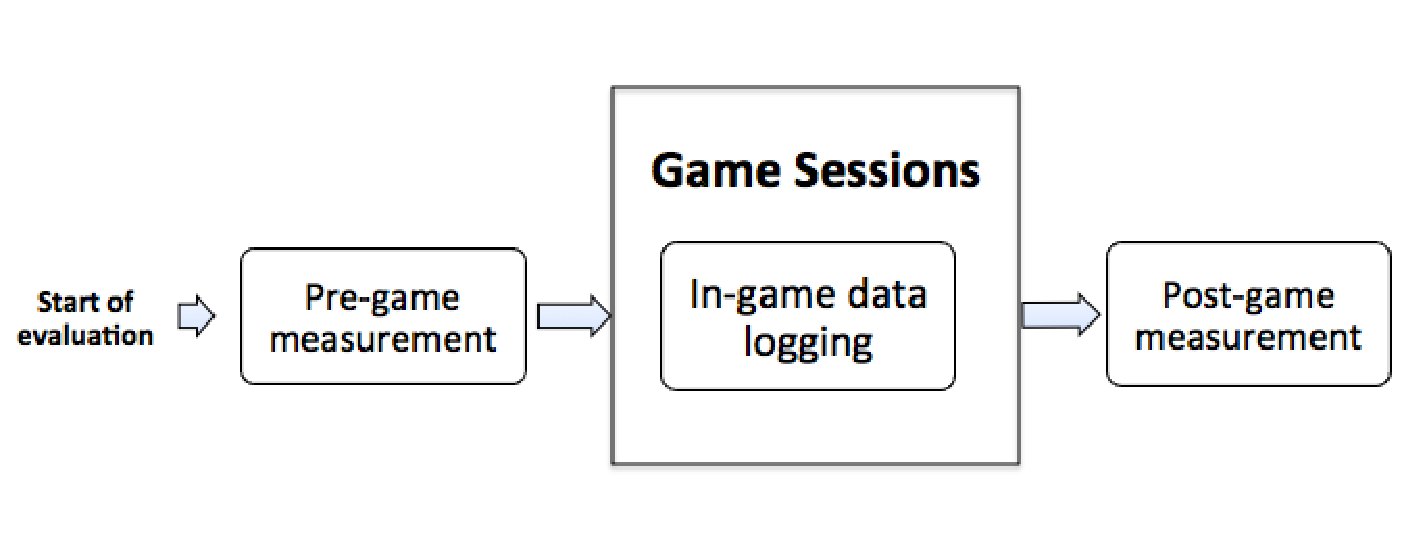
\includegraphics[width=3in]{pre-post-eval}
  \caption{Player Effectiveness Evaluation Process}
  \label{fig:pre-post-eval}
\end{figure}

\emph {(a) Literacy assessment:}
One important goal of the serious game for sustainability is the education effect on the players. Literacy assessment is an indicator of such effect if there is any.

This framework will use the similar approach described in \cite{csdl2-10-08} to assess the player's sustainability literacy. A set of literacy survey questionnaires (pre-game) will be presented to the players at the beginning of or before the game. After the game ends, the same survey (post-game) will then be presented to the players who responded the pre-game survey. These two set of survey response data will be compared to understand if there is any changes.

The extent of player's sustainability literacy change will indicate the degree of educational effectiveness of the serious game for sustainability.

\emph {(b) Behavior change assessment:}
Positive behavior change is another main goal of a serious game for sustainability. A serious game for sustainability normally include some degree of resource consumption measurement. This framework will use resource consumption data before and after the game as part of the assessment for the result of the player's sustainability behavior change.  The resource consumption baseline prior to the game will be established based on the history data. During and after the game, we can compare the resource consumption with the baseline for a particular day to understand to what extent the resource consumption has changed.

The problems with using the baseline to assess the energy reduction in the cases of dormitory energy challenge is discussed in details here\cite{csdl2-12-08}.
 As a framework for evaluating the effectiveness of serious game for sustainability in a broader context beyonds the dormitory challenge, we continue to use the baseline method as one way to assess the resource consumption reduction.

Besides using resource consumption change as one of the indicators of the player's behavior change, we also recommends to administrate behavior survey to the players, to understand the change (if there is any). A pre-game survey could be presented to the players to ask about their current sustainability behavior, then after the game, a post-game survey to ask about the player's behavior again. These two set of survey response data will be compared to understand if there is any changes.

The combination of resource consumption changes and self-reported behavior changes, will be used to understand the degree of behavior effectiveness of the serious game for sustainability.

\emph {(c) Engagement assessment:}
Player's engagement is an important assessment to understand the effectiveness of a serious game. By investigating the degree of engagement, we understand that the players are actively participating in the game thus any changes in the player's literacy and and behavior, are related to the participation in the game, although we can not theoretically prove that the participation cause the changes. On the other hand, if there is no or little participation, we could safely deduce that if there is any changes in sustainability literacy and behavior, they are mostly caused by something else, not the serious game in question.

A serious game should include detailed log data for the players' interaction with the game. These are the engagement metrics I propose to measure the player engagement for a serious games for sustainability:

\begin{itemize}
\item active participation rate
\item number of players per day
\item average session time
\item submissions per day
\item level of social engagement
\item website errors
\end{itemize}

\subsubsection{2. Game designer efficiency}
The research question to be investigated for the evaluation of game designer efficiency is: \emph{How efficient is it to design a game using the system?}

In order to investigate how efficient it is to design a game, we will look at how much time it takes to design the game, and how many errors the designers encountered during the design process.
The IT infrastructure for a serious game normally provide certain tools or interfaces for the designers to design the game. This may involve configuring global settings for the game, such as how long will the game run, who are the players, how to design individual game elements.

This framework proposes to first identify the list of design tasks, then look at two set of data to assess the game designer's efficiency. One set of data is the admin log data for the interaction between the game designer and the IT infrastructure interface. From these log data, we could derive the time it took a designer to complete a certain design task using the interface, and any system error he encountered. Another set of data could be obtained by interviewing the designers to answer:
\begin{itemize}
    \item How much time did you spend to complete each design task?
    \item What problem did you encountered?
    \item Did you find it difficult to configure? what is difficult?
    \item Did you find it difficult to design a specific game? which one, what is difficult?
    \item What did you like the least when using the system?
\end{itemize}

\subsubsection{3. Game manager efficiency}
The research question to be investigated for the evaluation of game manager efficiency is: \emph{How efficient is it to manage the game using the system?}

In order to investigate how efficient it is to manage a game, we will look at how much time it takes to manage the game, and how many errors the game managers encountered during the process.
The IT infrastructure for a serious game normally provide certain interfaces for the managers to manage the game. This may involve managing player submissions, monitoring the game state, entering manual resource data, notifying winners of the game, etc.

This framework proposes to first identify the list of managing tasks, then look at two set of data to assess the game manager's efficiency. One set of data is the admin log data for the interaction between the game manager and the IT infrastructure interface. From these log data, we could derive the time it took a manager to complete a certain managing task using the interface, and any system error he encountered. Another set of data could be obtained by interviewing the managers to answer:
\begin{itemize}
\item How much time did you spend to complete each managing task?
\item What problem did you encountered?
\item Did you find it difficult to manage? what is difficult?
\item What did you like the least when using the system?
\end{itemize}

It is possible that the same group of persons share the role of game manager and game designer, for example, the game designer also manages the game. In this case, the evaluation will look at the same person's data, both admin log and interview, with different assessing questions.

\subsubsection{4. System admin efficiency}
The research question to be investigated for the evaluation of system admin efficiency is: \emph{How efficient is it to install and maintain the system?}

In order to investigate how efficient it is to install and maintain the system, we will look at how much time it takes to install and maintain the system, and how many errors encountered during the process. This framework proposes to interview the system admin to answer:
\begin{itemize}
\item How much time did you spend to install the system?
\item How much time did you spend to maintain the system?
\item What problem did you encountered?
\item Did you find it difficult to admin the system? what is difficult?
\item What did you like the least about administrating the system?
\end{itemize}

\subsubsection{5. Developer efficiency}
The research question to be investigated for the evaluation of developer efficiency is: \emph{How efficient is it to understand, extend and debug the system?}

In order to investigate how efficient it is to understand, extend and debug the system, we will look at how much time it takes to install and maintain the system, and how many errors encountered during the process. This framework proposes to interview the developer to answer:
\begin{itemize}
\item How much time did you spend to set up the dev env?
\item How much time did you spend to develop and debug an enhancement?
\item What problem did you encountered?
\item Did you find it difficult to understand, extend and debug the system? what is difficult?
\item What did you like the least when developing with the system?
\end{itemize}

\subsubsection{6. Researcher efficiency}
The research question to be investigated for the evaluation of researcher efficiency is: \emph{How efficient is it to do research with the system?}

In order to investigate how efficient it is to do research with the system, we will look at how much time it takes to use the system for specific research query, and how many errors encountered during the process. This framework proposes to interview the researcher to answer:
\begin{itemize}
\item How much time did you spend to collect the research data for a specific topic?
\item What problem did you encountered when collecting the data?
\item Did you find the data you collect helpful to your research? if not, what can be improved?
\item Did you find it difficult to collect the data from the system? what is difficult?
\item What did you like the least about using the system?
\end{itemize}

\section{Case Study of Makahiki}
Now that we had described in full extent the SEE evaluation framework, this section will discuss the case study of how the SEE is applied to the Makahiki serious game framework for sustainability that we developed. First we will first explain what the Makahiki game engine is about.

\subsection{Makahiki in Brief}

We developed an innovated serious game framework for sustainability called Makahiki, as an IT infrastructure for the development of sustainability challenges. Makahiki explores one section of the design space
where virtual world game mechanics are employed to affect real world sustainability behaviors.

Makahiki consists of a configurable game engine that can be customized to the needs of different organizations.  It includes a library of pre-built game ``widgets'' that implement a variety of game mechanics.  Using the widgets, an organization can create a custom energy challenge in which players can compete individually and/or in teams to earn the most points by reducing their energy consumption as well as by learning about energy concepts in general. Figure \ref{fig:makahiki-architecture} illustrates the architecture of Makahiki. Figure \ref{fig:makahiki-games} shows a few examples of the games implemented in the Makahiki game library. More detailed description of Makahiki can be found here \cite{csdl2-12-06}.

\begin{figure}
  \center
  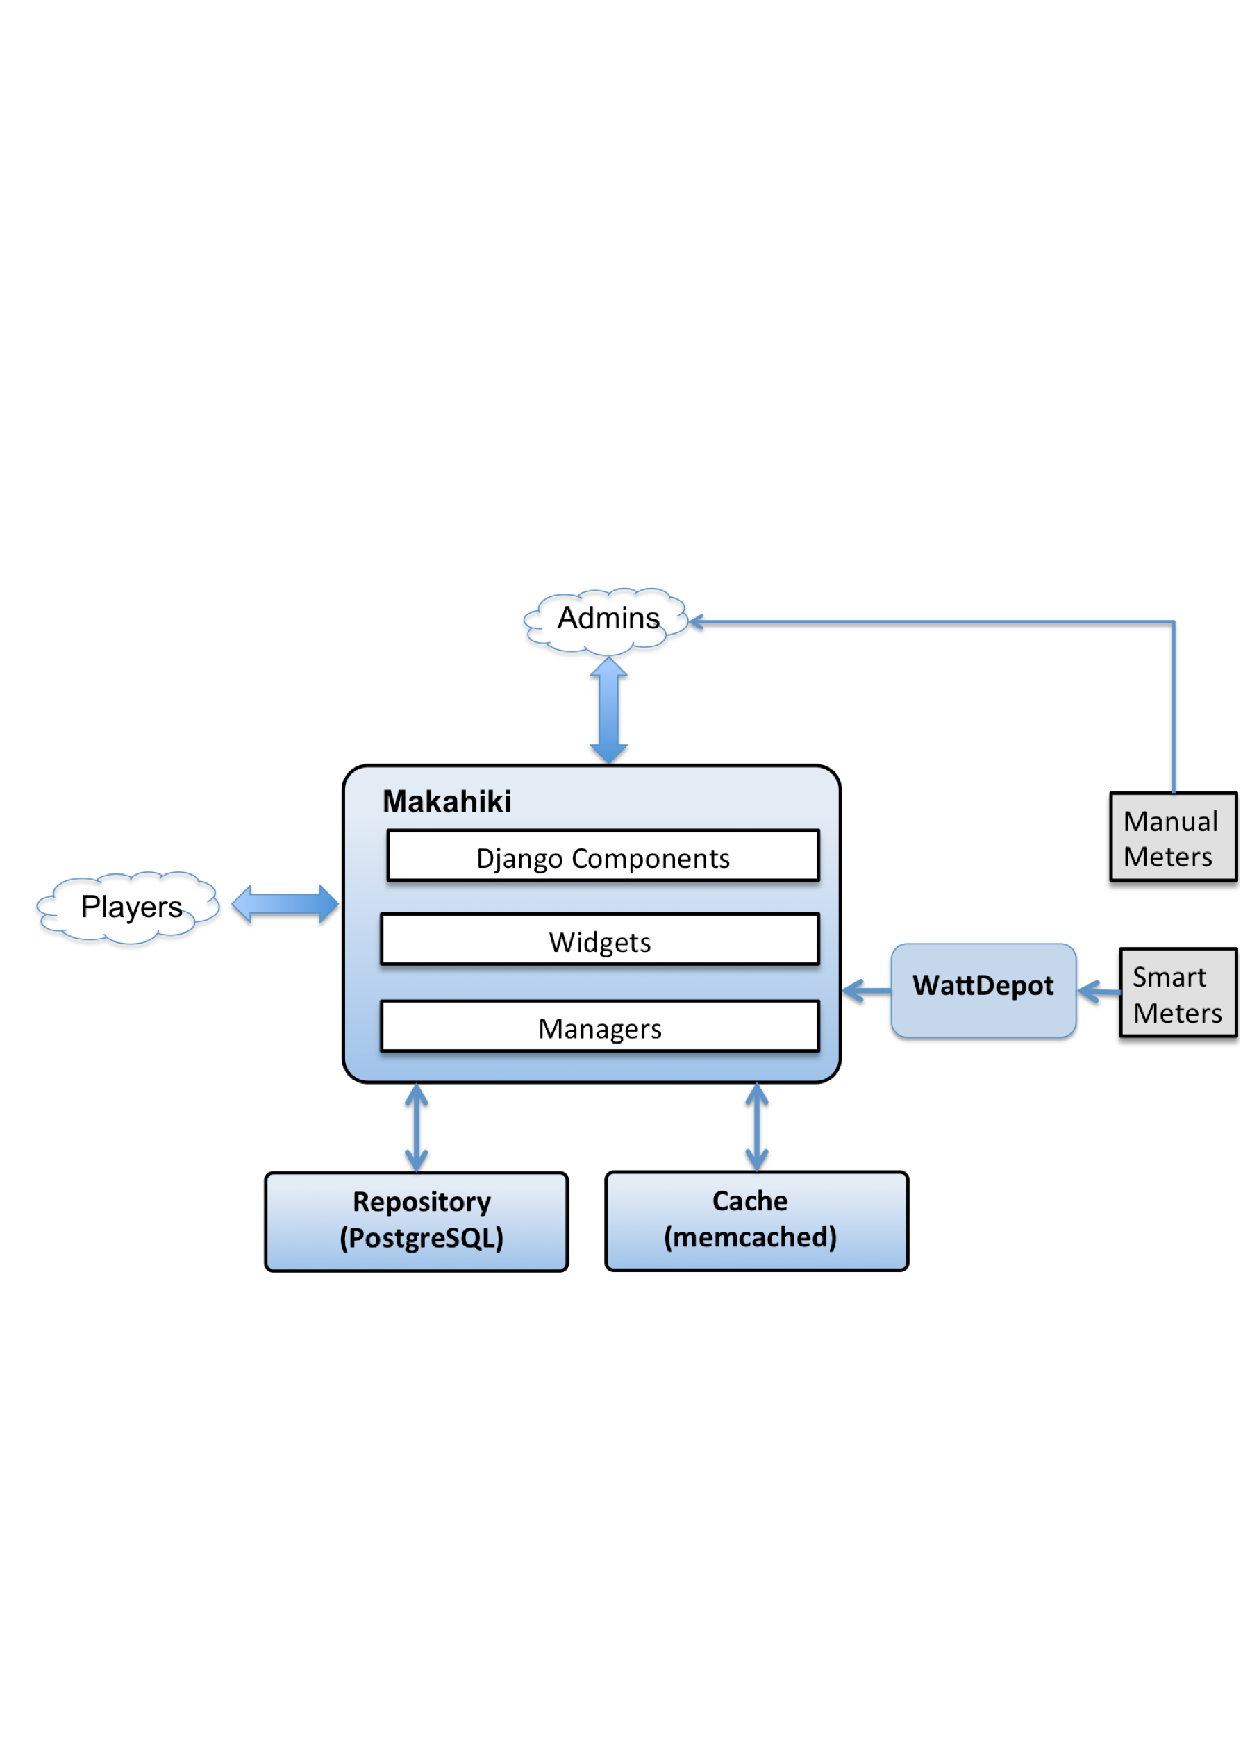
\includegraphics[width=3in]{makahiki-system-architecture}
  \caption{Architecture of Makahiki}
  \label{fig:makahiki-architecture}
\end{figure}

\begin{figure}
	\center
		\subfigure[Smart Grid Game]{\label{fig:SmartGrid}\includegraphics[width=1.5in,height=1.2in]{smart-grid-game.eps}}
		\subfigure[Energy Goal Game]{\label{fig:DailyEnergyGoal}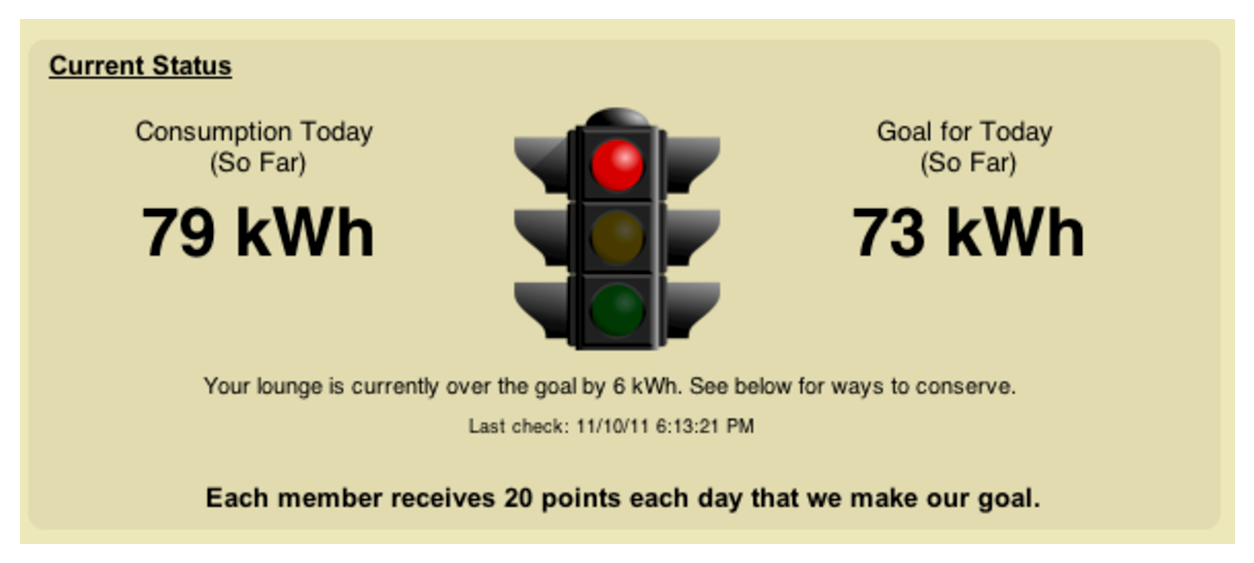
\includegraphics[width=1.5in,height=1.2in]{daily-energy-goal-game.eps}}
		\caption{Makahiki Game Library}
		\label{fig:makahiki-games}
\end{figure}

\subsection{Field studies}

As a serious game framework for sustainability, Makahiki had been used in the real world. In 2012, three different organizations used Makahiki to implement their own sustainability serious games called Kukui Cup challenge.

The first and second Kukui Cup Energy challenge of University of Hawaii was held in 2011 and 2012 for over 1,000 first year students living in the residence halls. Hawaii Pacific University (HPU) held a Kukui Cup Energy challenge in Fall 2012 for about 200 students. An international organization called the East-West Center (EWC) held a Kukui Cup Energy and Water challenge for the international residents living in the resident halls without smart meters, so the resource consumption data had to be entered by the game mangers manually.

The successful creation of serious game challenges by three different organizations provides evidence that the Makahiki serious game engine can be tailored to the differing needs of separate organizations. First, UH uses smart meters by Electro-Industries Inc., while HPU uses smart meters by EGauge Inc., and EWC collected their energy data manually. Second, while UH and HPU challenges involved only energy consumption data, the EWC challenge involved both energy and water consumption data (which was also collected manually).  Third, the IT infrastructure at UH and HPU provided authentication services using CAS and LDAP, while EWC used the built-in Django authentication. Fourth, the user interface was customized to ``brand'' each challenge with the logo, thematic elements, and the education contents of the sponsoring organizations.

Besides the real world usage of Makahiki in the series Kukui Cup challenge, We also performed in-lab evaluation experiments. Makahiki was used in the serious game development course at the Universiy of Hawaii. The students are seniors or graduate students majored in the computer science related fields. During the course, the students will install Makahiki, configure and design a serious game instance with Makahiki, and finally develop an enhancement to the Makahiki system. We asked the students taking the course to voluntarily participate in the evaluation experiments of Makahiki, using the SEE evaluation framework.

\subsection{Evaluation of Makahiki}
This section describes the details of Makahiki evaluation using the SEE evaluation framework.

\subsubsection{Player effectiveness}
Player effectiveness evaluation is performed using the Kukui Cup instance at the University of Hawaii at Manoa. There are over 1000 eligible players for this instances. They are the first year college student living in four similar structured resident halls in close vicinity. Makahiki system recorded detailed logging data from every interaction between the players and the website. The following engagement metrics are calculated based on the log data to assess the engagement level of instance:

\begin{itemize}
\item active participation rate
\item number of players per day
\item average session time
\item submissions per day
\item level of social engagement
\item website errors
\end{itemize}

In addition to the assessment of engagement metrics, we also administrated the two surveys, one before the challenge (pre-game) and one after the challenge (post-game). The survey is used to assess the effectiveness on player's sustainability literacy and behavior change.

The energy consumption data before, during and after the challenge are examined to understand any usage pattern or reduction during and after the challenge.

\subsubsection{System admin efficiency evaluation}

System admin efficiency evaluation is performed in the in-lab experiment. The students are tasked with installing the Makahiki system into their local computers as well as the cloud environment. In order to understand how much time it takes to install the Makahiki and what problems might be encountered, We designed a Google form which details the steps of installing Makahiki both locally and in the cloud, and for each step, we asked the students to record the time they spent and the problems they encountered.

Figure \ref{fig:makahiki-eval-form} illustrates a partial google form used for Makahiki system admin evaluation.

\begin{figure}[ht!]
   \centering
   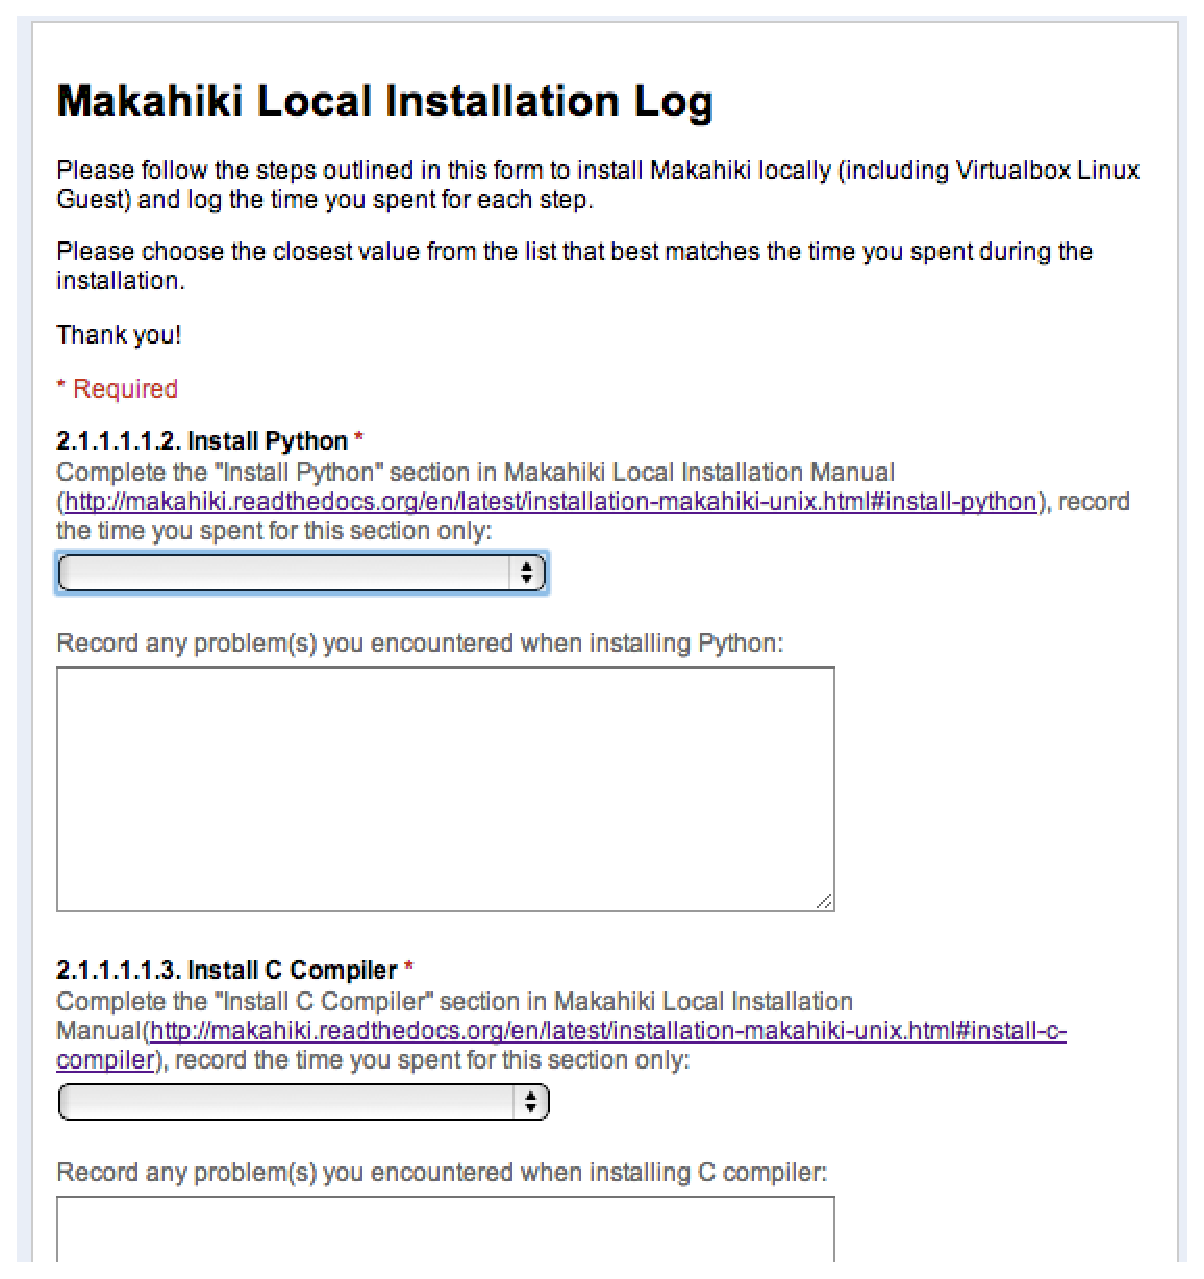
\includegraphics[width=3.5in]{developer-eval-form}
   \caption{Makahiki Evaluation Form}
   \label{fig:makahiki-eval-form}
\end{figure}

We also asked the students to provide feedback about their installation experiences in the form of blog post.

\subsubsection{Game designer efficiency evaluation}

Another class assignment for students is to design a Kukui Cup like serious game using Makahiki. We designed another google form to ask students to follow the designing steps and record their time and problem encountered during their designing process.

Students were also asked to provide feedback about their design experiences in the form of blog post.

Game designer efficiency evaluation is also performed by interviewing the game designers of the Hawaii Pacific University and East-West Center at Hawaii challenges. The interviews took place before the challenge starts to capture their experiences in using the Makahiki admin interface for the design process, which normally happen before the challenge. We analyzed both the qualitative data collected from the interviews and email changes with the game managers, and the quantitative collected from the admin interface log data.

\subsubsection{Game manager efficiency evaluation}
Game manager efficiency evaluation is performed by interviewing the game managers of the Hawaii Pacific University and East-West Center at Hawaii challenges. The interviews took place after the challenge. We asked them about their experiences in using the Makahiki admin interface for the managing process during the challenge. The admin interface log data is also analyzed to assess if there is any error encountered during the challenge management.

\subsubsection{Developer efficiency evaluation}

The students are tasked with developing an enhancement to the Makahiki instance. This involves setting up the development environment, following the tutorial to create the "Hello world" widget using Makahiki, and finally, develop the enhancement which extends the functionality of the Makahiki system.

The students are asked to submit their development source code to the public source code repository (Github) and write a blog post to discuss their efforts to complete the development activity.

We reviewed their source code to compare their code to the reference implementation, analyzed the blog post from the students, as well as any email correspondence from students discussing the problem in the development.

\subsubsection{Researcher experience evaluation}
We interviewed the researchers using the University of Hawaii instance.

\section{Future Work}
The design of SEE evaluation framework creates another research question: what are the strengths and weaknesses of this evaluation framework? To answer that question, we are planing to apply the evaluation framework to another serious game development environment (such as the commercial Lucid Dashboard system \cite{building-dashboard}). With the insights gained from another case study, the framework can be further improved.

One area of effectiveness evaluation is currently not addressed in the SEE framework: the longitudinal evaluation of player effectiveness.  We want to find out whether the serious game experience actually had lasting impacts on players. In the context of Makahiki-based serious games for sustainability, whether the student players were able to continue any positive sustainability behaviors after leaving their residence halls.

\section{Conclusion}
We proposed a serious game framework evaluation mechanism called Stakeholder Experience Evaluation (SEE). Six stakeholders' experiences, players, game designers, game managers, system admins, developers, researchers, are evaluated qualitatively and quantitatively to assess the extent of the effectiveness and efficiency of the serious game framework.

We also applied the SEE evaluation mechanism to the Makahiki serious game framework. The results show that ...

\section{Acknowledgments}
Omitted from review version.

%\textbf{Don't forget
%to acknowledge funding sources as well}, so you don't wind up
%having to correct it later.

% Balancing columns in a ref list is a bit of a pain because you
% either use a hack like flushend or balance, or manually insert
% a column break.  http://www.tex.ac.uk/cgi-bin/texfaq2html?label=balance
% multicols doesn't work because we're already in two-column mode,
% and flushend isn't awesome, so I choose balance.  See this
% for more info: http://cs.brown.edu/system/software/latex/doc/balance.pdf
%
% Note that in a perfect world balance wants to be in the first
% column of the last page.
%
% If balance doesn't work for you, you can remove that and
% hard-code a column break into the bbl file right before you
% submit:
%
% http://stackoverflow.com/questions/2149854/how-to-manually-equalize-columns-
% in-an-ieee-paper-if-using-bibtex
%
% Or, just remove \balance and give up on balancing the last page.
%
\balance

% If you want to use smaller typesetting for the reference list,
% uncomment the following line:
% \small
\bibliographystyle{acm-sigchi}
\bibliography{sustainability,csdl-trs,gamification,13-03}
\end{document}
